\documentclass[8pt]{article}
\usepackage[utf8]{inputenc}
\usepackage{soulutf8}

\usepackage{graphicx}
\usepackage{wrapfig}

\usepackage{pifont}
\usepackage{tgpagella}

\usepackage{hyperref}
\usepackage{multicol}
\usepackage{lipsum}
\usepackage[margin=1in]{geometry}
\setcounter{secnumdepth}{0}
\setlength\parindent{0pt}
\usepackage{float}

\usepackage{physics}

\usepackage{fancyhdr}
\pagestyle{fancy}
\lhead{Physics 181—Statistical Mechanics}
\rhead{Maggie Wang}

\usepackage{titlesec}
\usepackage{ulem}

\titleformat*{\section}{\Large\bfseries}
\titleformat{\subsection}{\bfseries}{\bfseries\thesubsection}{0.5em}{\ul}
\titleformat*{\subsubsection}{\small\bfseries\itshape}
\titleformat*{\paragraph}{\small\bfseries}
\titleformat*{\subparagraph}{\small\bfseries}

\titlespacing\section{0pt}{12pt plus 4pt minus 2pt}{3pt plus 2pt minus 2pt}
\titlespacing\subsection{0pt}{4pt plus 0pt minus 0pt}{4pt plus 0pt minus 0pt}
\titlespacing\subsubsection{0pt}{12pt plus 4pt minus 2pt}{0pt plus 2pt minus 2pt}


\title{Physics 181: Statistical Mechanics}
\author{Lectures and Content by Matthew Schwartz \\
Notes by Maggie Wang}
\date{Harvard University, Spring 2020}

\begin{document}

\small

\maketitle

\noindent Full course notes (2019): \url{http://users.physics.harvard.edu/~schwartz/teaching}.

% \maketoc
\begin{multicols*}{2}
  \tableofcontents
\end{multicols*}

\newpage

\newgeometry{top=1in,bottom=1in,right=0.4in,left=0.4in}
\fancyhfoffset[E,O]{0pt}

% \begin{multicols*}{2}

\twocolumn

\section{Lecture 1: Probability - 1/28}
TODO
\lipsum[1-3]

\section{Lecture 2: Diffusion - 1/30}
TODO
\lipsum[1-3]

\newpage

\section{Lecture 3: Equilibrium - 2/4}

% \subsection{Introduction}

% Postulate of equal a priori probabilities: in equilibrium, all possible states are equally likely.

% \textbf{Ideal gas}: interactions are short-ranged and collisions are elastic.

% \textbf{Phase space}: the set of allowed $\vec{q}_i$ and $\vec{p}_i$ for the $N$ particles. 6$N$ dimensional.

\subsection{Chaos}

\textbf{Chaotic}: uncontrollably sensitive to infinitesimal inaccuracies of the specifications of the system. The "butterfly effect". Property of systems w large DOF.

Molecules are hard spheres, radius $R$. Bounces off another sphere after traveling distance $l$ (mean free path). Deflects at angle $\theta$. $b$ is distance btwn sphere's centers perp to direction of motion.

\begin{figure}[h]
    \centering
    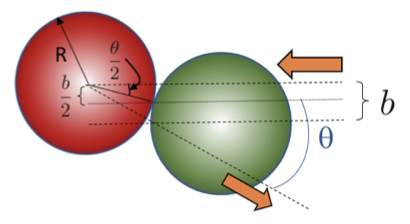
\includegraphics[width=0.7\linewidth]{figures/03_01.png}
\end{figure}

$\frac{b}{2} = R \sin \frac{\theta}{2}$

$\frac{b+ \Delta b_1}{2} = R \sin(\frac{\theta_1 + \Delta \theta_1}{2}) \approx R \sin(\frac{\theta_1}{2}) + R \frac{\Delta \theta_1}{2} \cos(\frac{\theta_1}{2}) + \cdots$

\begin{figure}[h]
    \centering
    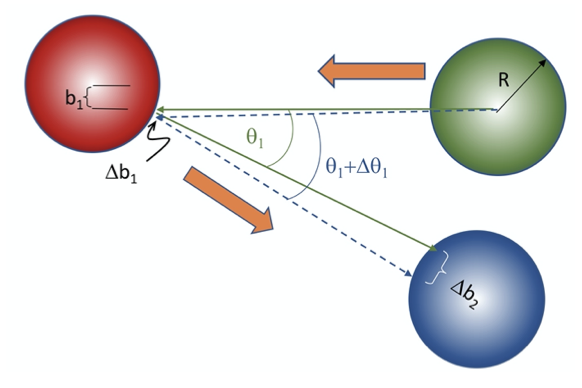
\includegraphics[width=0.8\linewidth]{figures/03_02.png}
\end{figure}

blah blah to do

After $N$ collisions, $\Delta \theta_N \approx (\frac{l}{R})^N \Delta \theta_1$. After just a few collisions, this factor can make small effects very very big.

Chaotic system: late time behavior is exponentially sensitive to initial conditions: changing the initial condition by a little bit has an enormous effect on the outcome.

\subsection{Maxwell and Molecular Chaos}

Systems tend towards flat probability distributions.

\subsubsection{Equilibration of molecular velocities}

Two random initial velocities are \textbf{uncorrelated}: $\langle \vec{v}_1 \cdot \vec{v}_2 \rangle = 0$.

The \textbf{average kinetic energy} of any molecular species in the gas is the same: $\langle m_1 \vec{v}_1^2 \rangle = \langle m_2 \vec{v}_2^2 \rangle$. Thus, heavier molecules move slower (on average) and average KE for any molecule is a universal quantity determined by the state of the gas, independent of the mass.

\subsubsection{Molecular chaos}

The \textbf{assumption of molecular chaos}: velocities of colliding particles are independent of each other, and independent of the position of the collision.

But, after a collision, two uncorrelated velocities become correlated.

\begin{figure}[h]
    \centering
    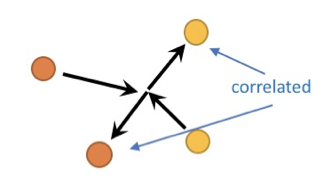
\includegraphics[width=0.4\linewidth]{figures/03_03.png}
\end{figure}

We should properly specify the state not as a point in phase space but as a region $R$ in phase space around the point $(p_i, q_i)$ of volume $\Delta V = (\Delta q)^{3N} (\Delta p)^{3N}$ with $\Delta q$ and $\Delta p$ our (classical uncertainty on the position and momentum.

After a short time, nearby points in phase space follow highly-correlated traj thru phase space.

\begin{figure}[h]
    \centering
    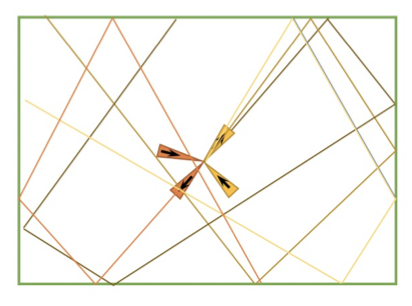
\includegraphics[width=0.5\linewidth]{figures/03_04.png}
\end{figure}

Over time, a phase space region $R$ of size $\Delta V$ fragments into an enormous number of small regions w the same total volume. When we course grain, the phase space volume increases (middle). Further time evolution with coarse graining fills up more and more of phase space.

\begin{figure}[h]
    \centering
    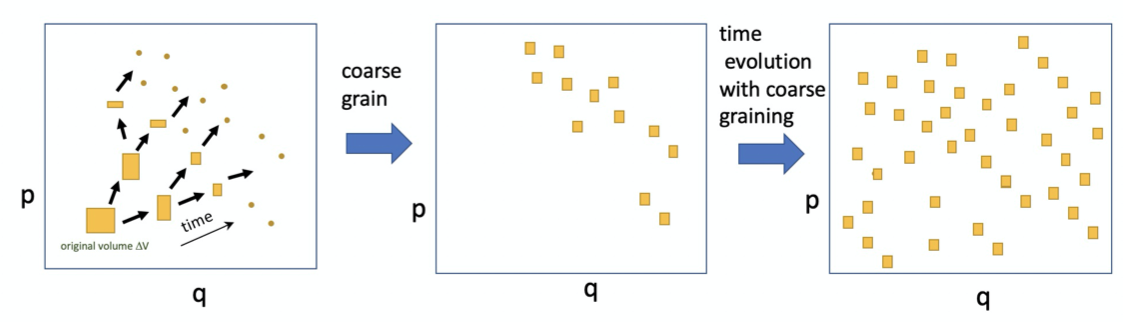
\includegraphics[width=1\linewidth]{figures/03_05.png}
\end{figure}

\textbf{Liouville's theorem}: sum of the phase-space volumes of all the fragments is the same as the original volume $\Delta V$ of the region $R$. This means the volumes of the fragments are getting smaller and smaller after each collision. 

We cannot possibly know what point in phase space our system is in with a precision better than $\Delta V$. So we must \textbf{coarse-grain} these small phase space volumes, treating them all the same way (cannot distinguish nearby points). Correlations are still there, but we cannot ever measure anything sensitive to them.

\subsection{Boltzmann's \textit{H} theorem}

\begin{align*}
    \dv{}{t}P_a(t) &= \sum_b P_b(t) T_{ba} - P_a(t) \sum_b T_{ab} \\
    &= \{\text{transitions } b \rightarrow a\} - \{\text{transitions } a \rightarrow b\}
\end{align*}

Assume all the $T_{ab} \neq 0$.

\textbf{The principle of detailed balance}: the transition rate from one state $a$ to $b$ is the same as the rate for $b$ going to $a$: $T_{ab} = T_{ba}$

It follows that $$\dv{}{t} P_a(t) = \sum_b T_{ab} [P_b(t) - P_a(t)]$$

If $P_a(t) > P_b(t)$ then $P_a(t)$ will go down, and if $P_b(t) > P_a(t)$ then $P_a(t)$ will go up. Thus over time, $\lim_{t \rightarrow \infty} P_a(t) = \lim_{t \rightarrow} P_b(t)$.

When there are $N$ states, we consider the quantity $H (t) = -\sum_a P_a(t) \ln P_a(t)$. math...

\textbf{Boltzmann H theorem}: $\dv{}{t} H(t) \geq 0$

Equilibrium is only possible if $\dv{}{t} H(t) = 0$, which only happens if $P_a(t) = P_b(t)$ for all states $a$ and $b$ (postulate of equal a priori probabilities).

\textbf{Loschmidt's paradox}: Boltzmann $H$ theorem is not time-reversal invariant: $H$ increases as we move forward in time, not backwards in time. Resolution: coarse-graining is not symmetric in time.

\subsection{The ergodic hypothesis}

\textbf{Ergodic system}: one for which the average over the set of possible states (the ensemble average) is the same as the average over time for a particular state (the time average). We can find the probabilities of a system being a state at a given time $t$ by looking at the possible states a system passes through time.

(a) is non-ergodic, since it would never reach ponts closer than a certain distance from the center. (b) is ergodic.
\begin{figure}[h]
    \centering
    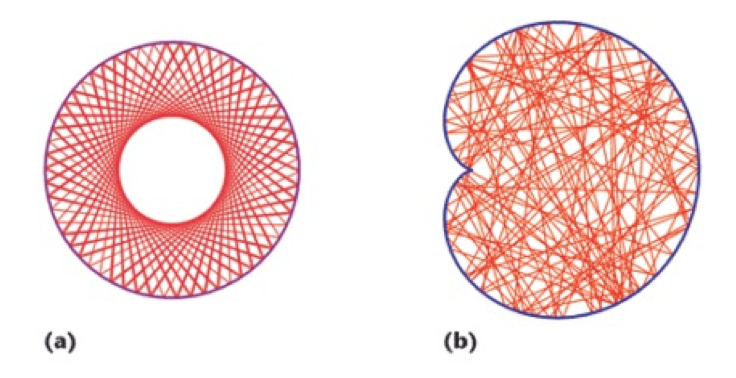
\includegraphics[width=0.8\linewidth]{figures/03_06.png}
\end{figure}

\subsection{Counting states}

\textbf{Postulate of equal a priori probabilities}: all accessible microstates are equally likely.

\textbf{Ideal gas}: all collisions are perfectly elastic

Number of states: $\Omega = \Omega_q \Omega_p$

$\Omega_q = [\frac{V}{(\Delta q)^3)}]^N$

$\Omega(N, V, E) = 2 e^{\frac{3}{2} N} (\frac{V}{\Delta q}{\Delta} p)^3)^N (\frac{4 \pi m E}{3N})^{\frac{3N}{2}}$

Number of states is an extremely rapidly growing function of energy: $\Omega(E) \sim E^{10^{24}}$

\subsection{Maxwell-Boltzmann distribution}

Velocity distribution of molecules in a gas.

$$\dv[3]{P(\vec{p})}{p} = (\frac{3}{4 \pi m \bar{\epsilon}})^{3/2} e^{-\frac{1}{\bar{\epsilon}} \frac{3 \vec{p}^2}{4 m}}$$

\textbf{Maxwell-Boltzmann distribution}: the distribution of velocities of gas molecules is computed by counting the number of ways the total energy of the gas can be distributed among the molecules.

\begin{figure}[h]
    \centering
    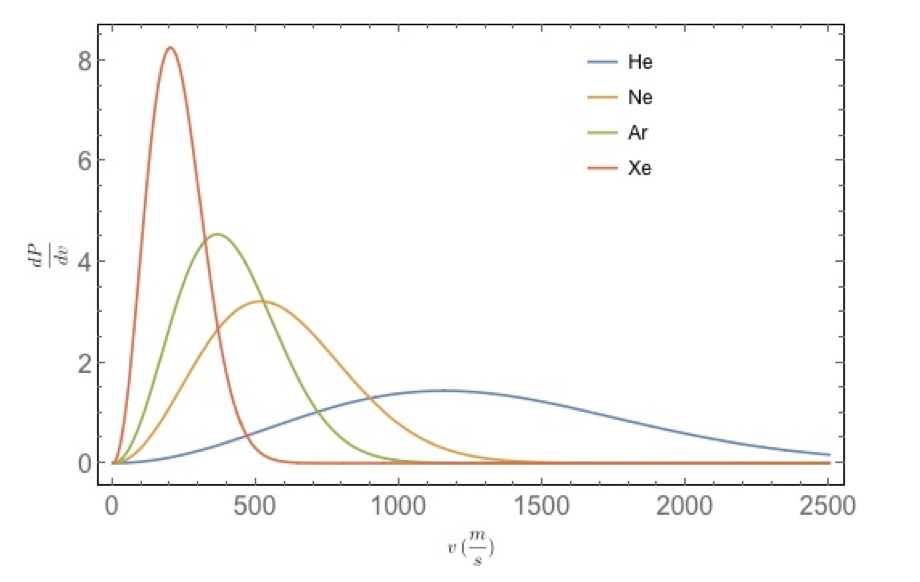
\includegraphics[width=0.8\linewidth]{figures/03_07.png}
\end{figure}

\end{document}
